The software landscape for fast algorithms is fragmented. Development  is split amongst a plurality of groups each operating siloed infrastructure. There are no parallel open-source softwares for the fast construction and use of strongly admissible $\mathcal{H}$ and $\mathcal{H}^2$ matrices for shared-memory systems. However, the `STRUMPACK' \cite{ghyselsstrumpack} package does offer an MPI accelerated HODLR and HSS matrix package. For $\mathcal{H}$ and $\mathcal{H}^2$ matrices, Ho et. al provide `FLAM' \cite{ho2020flam}, a multithreaded single node implementation of an alternative factorization based on `recursive skeletonisation'. We defer a discussion of recursive skeletonisation until section \ref{sec:3_2}, for our current purposes we can assume it's another hierarchical format for $\mathcal{H}^2$ which allows for $O(N)$ matrix vector products and inversions. In STRUMPACK, we use a HSS matrix approximation, as noted in \cite{yokota2015fast} this isn't strictly appropriate for (\ref{eq:two_box_calc:sec_1_2}) as it's a strongly admissable problem. Regardless of this, STRUMPACK offers an understanding of the performance of a highly optimised parallel algebraic solver. For FMMs the situation is better, with a greater number of open source projects in active development. The `Fast Algorithms' project\footnote{https://github.com/fastalgorithms} have developed multithreaded single-node analytical FMMs in $\mathbb{R}^2$and $\mathbb{R}^3$ \cite{fmm2d, fmm3d}. Another set of leading implementations are provided by the ExaFMM project\footnote{https://github.com/exafmm}, with the MPI accelerated analytical, `ExaFMM' \cite{exafmm}, and the multithreaded single-node kernel-independent FMM, `ExaFMM-T' \cite{wang2021exafmm}. All the above software, except FLAM, are written in either Fortran or C++. FLAM, written in Matlab, is not designed for high performance. However, it remains the only publicly available multithreaded implementation of fast algorithms for $\mathcal{H}^2$ matrices, and we include it for comparison.

We compare these softwares for the calculation of (\ref{eq:two_box_calc:sec_1_2}) with $N$ randomly distributed particles placed in a unit cube, $[0, 1]^3$, with uniform charge, $q_i=1$, in figure (\ref{fig:sec_2_1:software_comparison}). Experiments are taken on a single-node AMD Ryzen Threadripper 3970X 32 core Processor, with 250GB of memory. To avoid thread oversubscription in STRUMPACK and ExaFMM, both designed for multi-node systems, the maximum number of OpenMP threads is restricted to one. In comparing these softwares we aimed to emulate the workflow of a typical user evaluating the differences between software packages, and therefore restricted our study to runs which converged in less than $2 \times 10^3$ s. Figure (\ref{fig:sec_2_1:software_comparison}a) plots the time to compute (\ref{eq:two_box_calc:sec_1_2}), including the time to create all required data structures. For the algebraic softwares, FLAM and STRUMPACK, this includes the time to factorise and store an explicit matrix representation of (\ref{eq:two_box_calc:sec_1_2}). The factorization scales as $O(N^2)$ for both softwares, which lies in contrast with the linear scaling of their matrix vector products once factorised (fig. (\ref{fig:sec_2_1:software_comparison}c))s. We note that for STRUMPACK it is difficult to recover a linear scaling for the matrix vector product in our experiments as convergence times for moderate problem sizes, $N \geq 10^5$, exceeded $2 \times 10^3$ s. The algebraic software currently available in the open source is completely impractical for computing even moderately sized matrix vector products, i.e. $N=O(10^6)$. One might argue that their expensive factorization cost is worth it if one proceeds to compute (\ref{eq:two_box_calc:sec_1_2}) multiple times, or if one wants to quickly find an inverse. However, the FMM softwares tested beat both algebraic softwares by several orders of magnitude, making it much more tenable to apply them multiple times if required, and to find matrix inverses via an iterative Krylov type methods.

\begin{figure}
    \begin{tabular}{cc}
        \subfloat[\centering Runtime]{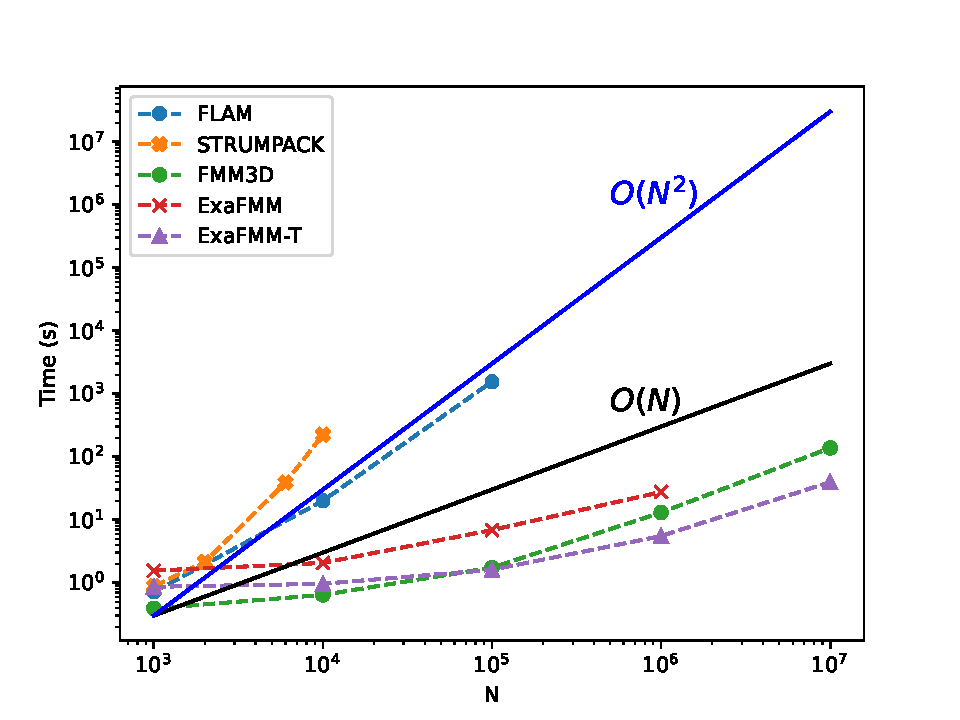
\includegraphics[width=75mm]{ch_2/runtime.pdf}} & \subfloat[\centering Peak memory]{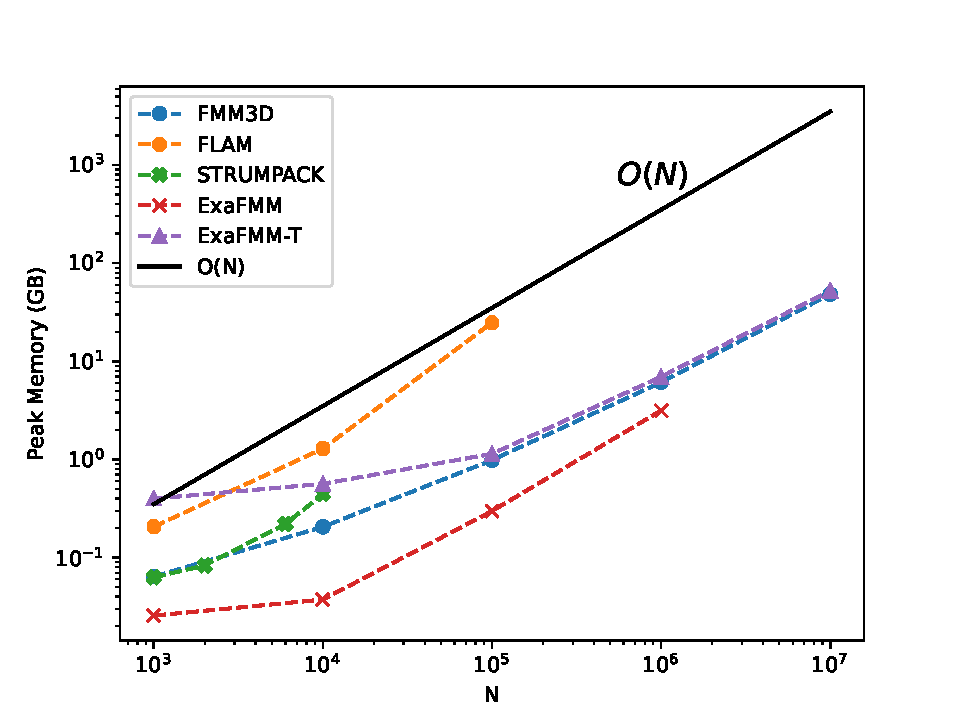
\includegraphics[width=75mm]{ch_2/memory.pdf}}
    \end{tabular}
    \centering \subfloat[\centering Matrix vector product time for algebraic methods.]{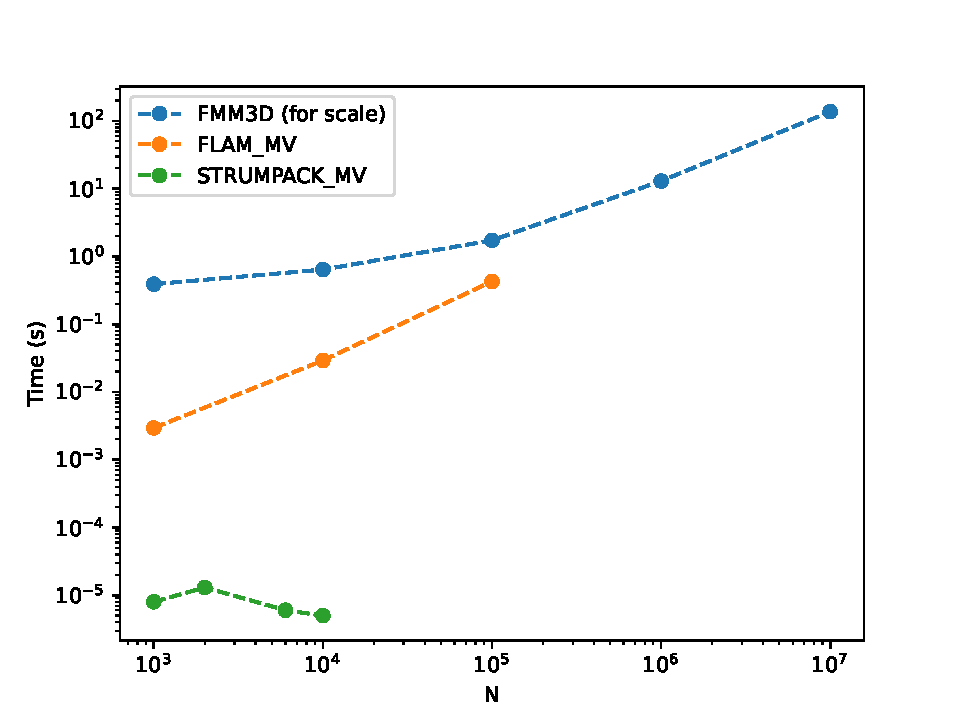
\includegraphics[width=75mm]{ch_2/alg_matvec.pdf}}
    \caption{Comparison of parallel software for fast algorithms, used to caclulate (\ref{eq:two_box_calc:sec_1_2}). Simulations were compared for convergence times $\leq 2 \times 10^3$ s.}
    \label{fig:sec_2_1:software_comparison}%
\end{figure}

The FMM softwares also appear to exhibit markedly different behaviours from each other, which are difficult to explain with purely theoretical considerations. Each is run with an expansion order $P=10$, as expected from theory the analytical FMMs, ExaFMM and FMM3D, consume less memory than the kernel-independent ExaFMM-T (fig. (\ref{fig:sec_2_1:software_comparison}b)). However, for larger problem sizes this difference is marginal between FMM3D and ExaFMM-T. For the largest problem size tested, $N=10^7$, ExaFMM-T is roughly 3.5 times faster than FMM3D with a similar memory footprint. Strangely the analytical ExaFMM fails to converge for $N=10^7$, as its memory requirements exceed 250 GB. Each software implements numerous techniques for acceleration, however these don't necessarily overlap. ExaFMM-T for example uses optimized algorithms for the calculation of inverse square roots \cite{malhotra2015pvfmm}, as well as using SIMD vectorisation with SSE/AVX and AVX-512 compatibility. Similarly by stacking $T^{M2L}$ as in (\ref{eq:sec_1_2:m2l_stacked}), they optimise cache-reuse \cite{wang2021exafmm}. However, FMM3D and ExaFMM are presented opaquely to users, with little openly available documentation of their optimisations.

Another point of difference between the softwares is in their usability, defined by the ease with which one can install software in different environments, and learn about its API. This important work is often dismissed as mere software engineering, but it is as crucial for the dissemination and uptake of scientific software as raw performance. Of the softwares tested, FMM3D and ExaFMM-T standout with publicly available websites documenting their installation and APIs, code examples, as well as bindings to higher level languages such as Python, Julia and Matlab. This lies in contrast to ExaFMM, which is poorly documented, and clearly still an `alpha' project, not ready for wide scale distribution. STRUMPACK, though relatively well documented, does not support wrappers to higher-level languages. Written in C++, its documentation is largely a description of its object hierarchy, with few examples documenting real world use cases.

- large number of projects, not clear how they map from theory. 

- unclear whether differences are implementational or due to underlying algorithm

- publicly available literature doesn't make it clear which software can do what problem. 

- many/most don't document their optimisations

- often no bindings to other languages.

- no high performance library for algebraic methods, that's good and extends to $\mathcal{H}$/$\mathcal{H}$ matrices

- No overlap between software projects has lead to redundant development of high performance optimisations.

- Building codes is not all easy. STRUMPACK, distribution via spack, but otherwise large list of custom dependencies. Traditional C++ dependency hell to get set up. Other software isn't designed for high-performance, and distributed with custom instructions to build from source. SPACK packages, need to look into how they are made and how easy they are to distribute.

- JIT compilers, and the rise of performant development in higher level languages. Can we develop an ergonomic FMM? source code all in Python? ... Next chapter.

- If not Python then what? C++ projects have a documented history of overcomplicating data structures. We want it to be as usable as possible, with few complex hierarchies, and designed for data oriented design (vis object oriented design). 